
\subsection{Polynomial Encoding}
\label{sec:encoding}
At the heart of our protocol is an encoding of integer polynomials with bounded coefficients as integers with useful homomorphic properties. To extend the encoding to polynomials over an odd prime field $\mathbb{F}_p$, we first lift them to the ring of polynomials over the integers by selecting representatives from $[-\frac{p-1}{2},  \frac{p-1}{2}]$ for each coefficient. The lifted polynomial has bounded integer coefficients and can hence be mapped into the integers.

We write $\ZZ(b):=\{x \in \ZZ \, | \, \vert x \vert  \leq b\}$ as the set of integers with absolute value less than or equal to $b$. In a slight abuse of notation we write $\ZZ(b)[X]\subset \mathbb{Z}[X]$ as the set of integer polynomials with bounded coefficients. 

\paragraph{Encoding}
For a ``large'' integer $q$, the map $\mathsf{Enc} : \mathbb{Z}((q-1)/2)[X] \rightarrow \mathbb{Z}, \, f(X) \mapsto f(q)$ is an injective map from the domain of polynomials with bounded coefficients to the integers. This means the map can be used as encoding of polynomials in the domain $\ZZ(b)[X]$ with $b<q/2$.
\paragraph{Decoding}
Decoding works as follows. Define the partial sum $S_k := \sum_{i=0}^k f_i q^i$ with $S_{-1} := 0$ and observe that when $(S_k \bmod q^{k+1}) > q^{k+1}/2$ then $S_k < 0$ whereas when $(S_k \bmod q^{k+1}) < q^{k+1}/2$ then $S_k \geq 0$. 
So when decoding $y \in \mathbb{Z}$, we can get $S_k$ for any $k$ by setting $S_k$ to $y \bmod q^{k+1}$ if $y \bmod q^{k+1}$ is less than $\frac{q^{k+1}}{2}$ or to $q^{k+1}- (y \bmod q^{k+1})$ otherwise.
Two consecutive partial sums yield a coefficient of $f(X)$: $f_k = \frac{S_{k} - S_{k-1}}{q^{k}} \in \ZZ(b)$. These operations give rise to the following algorithm.\\
\begin{minipage}{\textwidth}
\begin{mdframed}
\begin{flushleft}
	$\pro{Dec}(y \in \mathbb{Z}):$
	\begin{enumerate}[nolistsep]
	    \item \textbf{for each} $k$ \textbf{in} $[0, \, \lfloor \log_q(|y|)\rfloor]$ \textbf{do:}\\
		\item \pcind[1] $S_{k-1} \gets (y \bmod q^{k})$
		\item \pcind[1] \pcif{$S_{k-1} > q^{k}/2$} \textbf{then} $S_{k-1} \gets q^{k}-S_{k-1}$ \textbf{end if}
		\item \pcind[1] $S_k \gets (y \bmod q^{k+1})$
		\item \pcind[1] \pcif{$S_{k} > q^{k+1}/2$} \textbf{then} $S_{k} \gets q^{k+1}-S_{k}$ \textbf{end if}
		\item \pcind[1] $f_k \gets (S_{k} - S_{k-1}) / q^k$
		\item \pcreturn $f(X) = \sum_{i=0}^{\lfloor \log_q(|y|)\rfloor} f_i X^i$
	\end{enumerate} 
\end{flushleft}
\end{mdframed}
\end{minipage}

\begin{fact}
	The encoding scheme is uniquely decodable for polynomials in $\ZZ(b)[X]$ if $b<q/2$.
\end{fact}
The fact follows from $f(q)\in \ZZ$ being a unique integer representation of polynomials with coefficients bounded in absolute value by $b$ such that $b<q/2$. In particular for any partial sum $S_i$ we have $|S_i|<\frac{q^{i+1}}{2}$. From this it follows that $S_i-S_{k-i}=f_i \cdot q^i$.  

Note that the encoding has limited homomorphic properties: $\enc(g(X))+\enc(h(X))=\enc(g(X)+h(X))$ if $g(X)+h(X)\in \ZZ(b)$, \emph{i.e.}, if all its coefficients are less than $q/2$ in absolute value. This constraint is satisfied for example if the coefficients of $g$ and $h$ are less than $q/4$ in magnitude. Additionally, $\enc(g(X))\cdot \enc(h(X))=\enc(g(X)\cdot h(X))$ if $g(X)\cdot h(X)\in \ZZ(b)$.

\paragraph{Encoding of dyadic rational polynomials.}
In class groups there exists an algorithm to compute square roots of any element originally described by Gauß (modern description by Bosma and Stevenhagen~\cite{jtn/BosSte96}). As a result, in class groups an adversary can also commit to \defn{dyadic rationals} $\mathbb{D}:=\{\frac{x}{2^k} : \ x \in \ZZ \wedge k \in \NN\}\subset \QQ$, in addition to integers. When using class groups we therefore need to extend the encoding scheme accordingly. 

The encoding map is identical, except lifted to the dyadic rationals: $\mathsf{Enc} : \mathbb{D}[X] \rightarrow \mathbb{D}, \, g(X) \mapsto g(q)$. The main difference with respect to the integer encoding scheme will be that decoding works for dyadic rationals where \emph{both the numerator and the denominator are bounded}. Let $N \in \NN$ be a bound on the absolute value of the numerator and $2^D\in \NN$ be a bound on the value of the denominator, and let $\mathbb{D}(N, D) :=\{\frac{x}{2^a} \in \mathbb{D} : \ |x|\leq N \wedge 2^a \leq D\}$ denote the set of such bounded dyadic rationals. The encoding scheme is uniquely decodable if $N \cdot 2^a < q/2$.
 
Note that denominator of $g(q)$ is bounded by $2^{\lfloor\log_2(D)\rfloor}$, $D$ rounded down to the next power of $2$. To decode such a dyadic rational, compute the integer $y \gets g(q) \cdot 2^{\lfloor\log_2(D)\rfloor}\in \ZZ$  and use the decoding algorithm described above to decode a polynomial $f(X)$ in $\ZZ(q/2)[X]$. From $f(X)$ one derives the polynomial  $g(X) \gets \frac{f(X)}{2^{\lfloor\log_2(D)\rfloor}} \in \mathbb{D}(\lceil q/(2D)\rceil, 2^{\lfloor\log_2(D)\rfloor})[X]$ through division. If the integer polynomial encoding is uniquely decodable, then so is the scheme for dyadic rational polynomials. If $q$ is a power of $2$, then an adversary can encode Laurent polynomials, \emph{i.e.}, polynomials where some terms have negative powers. In order to disallow negative powers, $q$ must be odd.

\subsection{Information-Theoretic Polynomial Commitment Scheme}

Before we present our concrete polynomial commitment scheme based on groups of unknown order, we present an abstraction thereof that hides the concrete cryptographic steps. The purpose of this abstraction is two-fold: first, it provides an intuitive stepping stone from which presenting and studying the concrete cryptographic protocol is easier; and second, it opens the door to alternative cryptographic instantiations that provide the same interface but based on alternative hardness assumptions.

Let $[\![ \cdot ]\!] : \mathbb{Z}_p[X] \rightarrow \mathbb{S}$ be a homomorphic commitment function that sends polynomials over a prime field to elements of some set $\mathbb{S}$. Moreover, let $\mathbb{S}$ be equipped with operations $* + * : \mathbb{S} \times \mathbb{S} \rightarrow \mathbb{S}$ and $ * \cdot * : \mathbb{Z}_p[X] \times \mathbb{S} \rightarrow \mathbb{S}$ that accommodate two homomorphisms for $[\![ \cdot ]\!]$:
\begin{itemize}[nolistsep]
    \item a \emph{linear homomorphism}: $a \cdot [\![f(X)]\!] + b \cdot [\![g(X)]\!] = [\![af(X) + bg(X)]\!]$
    \item a \emph{monomial homomorphism}: $X^d \cdot [\![f(X)]\!] = [\![X^d f(X)]\!]$.
\end{itemize}
For now, assume both prover and verifier have oracle access to the function $[\![\cdot]\!]$ and to the operations $ * \cdot *$ and $* + *$. (Later on, we will instantiate this commitment function using groups of unknown order and the integer encoding of polynomials.)

%With this homomorphic commitment function and with the integer encoding scheme of the previous subsection, we construct a commitment function to polynomials that sends $\mathbb{Z}_p \rightarrow \mathbb{S}, f(X) \mapsto [\![f(q)]\!]$. This commitment function inherits the homomorphic properties of the integer encoding for a limited number of additions and multiplications-by-constant. With this commitment function we are in a position to present the abstract evaluation protocol.

The core idea of the evaluation protocol is to reduce the statement that is being proved from one about a polynomial $f(X)$ of degree $d$ and its evaluation $y = f(z)$, to one about a polynomial $f'(X)$ of degree $d'=\lfloor\frac{d}{2}\rfloor$ and its evaluation $y' = f'(z)$. For simplicity, assume that $d+1$ is a power of $2$.
The prover splits $f(X)$ into $f_L(X)$ and $f_R(X)$ such that $f(X) = f_L(X) + X^{d'+1} f_R(X)$ and such that both halves have degree at most $d'$. The prover obtains a random challenge $\alpha \in  \mathbb{Z}_p$ from the verifier and proceeds to prove that $f'(X)=\alpha \cdot f_L(X) + f_R(X)$ has degree $d'$ and that $f'(z) = y' = \alpha y_L + y_R$ with $y_L = f_L(z)$ and $y_R = f_R(z)$. 

The proof recursively repeats this reduction by using $f'(X),z,y'$ and $d'$ as the input. In the final step, $f(X) = f$ is a constant and the verifier checks that $f=y$.% $f \equiv y \bmod p$. Note that $|f| <  (\frac{p}{2})^{\log_2(d+1)+1}$ so a representation of $f$ requires at most $\lceil \log_2(d+1) \cdot \log_2(p)\rceil$ bits.

The commitment function binds the prover to one particular polynomial for every commitment held by the verifier. In particular, at the start of every recursion step, the verifier is in possession of a commitment $[\![f(X)]\!]$ to $f(X)$. The prover provides commitments $[\![f_L(X)]\!]$ and $[\![f_R(X)]\!]$, and the verifier checks their soundness homomorphically via $[\![f(X)]\!] = [\![f_L(X)]\!] + X^{d'+1} \! \cdot \! [\![f_R(X)]\!]$. From these commitments, the verifier can also compute the commitment to $f'(X)$ homomorphically, via $[\![f'(X)]\!] = \alpha \! \cdot \! [\![f_L(X)]\!] + [\![f_R(X)]\!]$. In the last step, the verifier checks that the constant polynomial $f$ matches the commitment by computing $[\![f]\!]$ outright. 

\begin{comment}
These operations give rise to the following informal, diagrammatic description of the \eval protocol.

\begin{figure}[!ht]
\begin{mdframed}[userdefinedwidth=\textwidth]
\newcommand{\dollar}{\$}
\begin{minipage}{\textwidth}
	\begin{flushleft}
	(Information-theoretic-)$\pro{Eval}([\![f(X)]\!], z, y, d; f(X)):$
		\begin{itemize}[nolistsep]
			\item \textbf{if} $d = 0$ \textbf{then:}
			\item[] \begin{tikzpicture}
			\node[] (prover) at (-5, 0) {\prover};
			\node[] (verifier) at (5, 0) {\verifier};
			\draw[->] (-4, -1) -- (4, -1) node[above, midway] {$f = f(X)$};
			\node[anchor=north west, xshift=-2.5cm, yshift=-1cm] (verifier checks) at (verifier.south west) {\begin{tabular}{l}
				check $f \in \mathbb{Z}_p$ and $f = y$ \\
				and $[\![f]\!] = [\![f(X)]\!]$
			\end{tabular}};
			\end{tikzpicture}
			\item \textbf{if} $d > 0$ \textbf{then:}
		 	\begin{tikzpicture}
			\node[] (prover) at (-5, 0) {\prover};
			\node[] (verifier) at (5, 0) {\verifier};
			\node[anchor=north west] (prover computes) at (prover.south west) {\begin{tabular}{l}
				split $f(X)$ into $f_L(X)$ and $f_R(X)$ \\
				s.t. $f(X) = f_L(X) + X^{d'+1}f_R(X)$ \\
				compute $y_L \gets f_L(z)$ and $y_R \gets f_R(z)$
			\end{tabular}};
			\draw[->] (-4, -2.7) -- (4, -2.7) node[above, midway] {$y_L, y_R, [\![f_L(X)]\!], [\![f_R(X)]\!]$};
			\node[anchor=north west, xshift=-2.5cm, yshift=-2.5cm] (verifier checks) at (verifier.south west) {\begin{tabular}{l}
			check $[\![f(X)]\!] =$ \\
			 $[\![f_L(X)]\!] + X^{d'+1}\cdot [\![f_R(X)]\!]$ \\
			check $y = y_L + z^{d'+1}y_R$ \\
			sample $\alpha \xleftarrow{\dollar} \mathbb{Z}_p$
			\end{tabular}};
			\draw[->] (4, -5.5) -- (-4, -5.5) node[above, midway] {$\alpha$};
			\node[anchor=north west, yshift=-0.5cm] (verifier updates) at (verifier checks.south west) {\begin{tabular}{l}
				compute $y' \gets \alpha y_L + y_R$ \\
				compute $[\![f'(X)]\!] \gets$ \\
				$\alpha \cdot [\![f_L(X)]\!] + [\![f_R(X)]\!]$
			\end{tabular}};
			\node[anchor=north west, yshift=-4cm] (prover updates) at (prover computes.south west) {compute $f'(X) \gets \alpha f_L(X) + f_R(X)$};
			\draw[<->] (4, -8) -- (-4, -8) node[above, midway] {run $\eval([\![f'(X)]\!], z, y', d'; f'(X))$};
			\end{tikzpicture}
		\end{itemize}
		\end{flushleft}
\end{minipage}
\end{mdframed}
\end{figure}
\end{comment}

\begin{comment}
These operations give rise to the following informal pseudocode description of the \eval protocol.
\begin{mdframed}
Information-theoretic $\eval$ protocol, informal. \\
Common knowledge: $[\![f(X)]\!], y, z, d$ \\
Secret knowledge for \prover: $f(X)$ of degree $d$ \\
Statement: $y = f(z) \bmod p$ and $\deg(f(X)) = d$
	\begin{itemize}[nolistsep]
	    \item \textbf{if} $d > 0$ \textbf{then:}
		\item \pcind[1] \prover splits $f(X)$ into polynomials $f_L(X)$ and $f_R(X)$ of degree $d'=\frac{d+1}{2}-1$ such that $f(X) = f_L(X) + X^{d'+1}f_R(X)$
		\item \pcind[1] \prover sends $[\![f_L(q)]\!]$ and $[\![f_R(q)]\!]$ as well as $y_L \gets f_L(z) \bmod p$ and $y_R \gets f_R(z) \bmod p$ to \verifier
		\item \pcind[1] \verifier checks that $[\![f_L(q)]\!]+q^{d'+1} [\![f_R(q)]\!] = [\![f(q)]\!]$ and $y_L+z^{d'+1} y_R =y$
		\item \pcind[1] \verifier sends a random challenge $\alpha$ from $[-\frac{p-1}{2} ; \frac{p-1}{2}]$ to \prover
		\item \pcind[1] \prover and \verifier recurse on $[\![f'(q)]\!]=\alpha [\![f_L(q)]\!]+[\![f_R(q)]\!]$ for the statement $f'(z) = \alpha y_L + y_R \bmod p$ and $\deg(f'(X)) = d'$
		\item \textbf{if} $d=0$ \textbf{then:}
		\item \pcind[1] $\prover$ sends the constant $f$ to $\verifier$
		\item \pcind[1] $\verifier$ checks that $f$ is a small constant, that $[\![\cdot]\!]$ evaluated in $f$ equals $[\![f]\!]$, and that $y = f \bmod p$
	\end{itemize}
\end{mdframed}
\end{comment}

\subsection{Concrete Polynomial Commitment Scheme}

We now instantiate the abstract homomorphic commitment function $[\![ \cdot ]\!]$. To this end we sample a group of unknown order $\mathbb{G}$, and sample a random element $\gr{g}$ from this group. 
We first lift the field polynomial $f(X)\in \ZZ_p[X]$ to an integer polynomial with bounded coefficients, i.e. $\hat{f}(X)\in \ZZ(\frac{p-1}{2})[X]$ such that $\hat{f}(X)\bmod p=f(x)$.
We encode $\hat{f}(X)$ as an integers by evaluating them at a ``large enough'' integer $q$. Finally we use exponentiation in $\GG$ to commit to the integer. $[\![f(X)]\!]$, therefore, corresponds to $\gr{g}^{f(q)}$. This commitment function inherits the homomorphic properties of the integer encoding for a limited number of additions and multiplications-by-constant. The monomial homomorphism for $X^d$ is achieved by raising the group element to the power $q^{d}$. To maintain consistency between the prover's witness polynomials and the verifier's commitments, the prover operates on $\hat{f}(X)$ as an integer polynomial rather than reducing modulo $p$.

The $\setup, \pro{Commit}$ and $\open$ functionalities are presented formally below. Note that the scheme is parameterized by $p$ and $q$; these values are determined by the context and independently of $\setup$.

%We now present our main technical contribution: a polynomial commitment scheme with an efficient evaluation protocol based on a group of unknown order $\GG$. For polynomials of degree $d=\poly$ the evaluation protocol uses $1+\lceil\log_2(d+1)\rceil$ rounds and $O(\log(d))$ communication and verifier work.

%Exponentiation in groups of unknown order is a succinct and homomorphic cryptographic commitments to an integer.
%Using the integer encoding of polynomials, or their encoding as dyadic rationals, above we can simply commit to a polynomial $f(X)$ with bounded coefficients by computing $\gr{g}^{f(q)} \in \GG$. Every polynomial in $\ZZ_p[X]$ naturally maps to an integer polynomial with coefficients in $B_{\frac{p-1}{2}}$. The commitment scheme, therefore, supports committing to polynomials in $\ZZ_p[X]$ for $p \leq q$. Interestingly, neither $p$ nor the degree $d$ need to be specified in the setup. 

%As long as $q$ and ``big enough'' they can be freely chosen.\alan{Todo: make this observation elsewhere.} %In class groups there is an efficient algorithm to compute square roots, and as a result, a prover can also commit to dyadic rationals. Since every dyadic rational corresponds to a unique element in $\ZZ_p$ we can simply extend the encoding to work for polynomials with bounded dyadic rational coefficients. The only difference is that we require $q$ to be odd such that the prover cannot commit to polynomials with negative powers. We will discuss the relationship between $p$, $d$ and $q$ in more detail later but first we describe the setup, commitment and opening algorithms:
\begin{small}
\begin{mdframed}[userdefinedwidth=\textwidth]
\begin{minipage}{\textwidth}
	\begin{flushleft}
	$\pro{Setup}(1^\secpar):$
		\begin{enumerate}[nolistsep]
			\item $ \GG \sample \ggen(\secpar)$
			\item $ \gr{g} \sample \GG$
			%\item $q \gets 2^k$ such that $q > (d+1) \cdot 2\cdot p^{\log_2(d+1)+1} $
			%\item Pick a prime $p\in \NN$ such that $\lceil\log_2(p)\rceil=\lambda$.
			%\item Pick a sufficiently large and odd $q\in \NN$ (See discussion above)
			%\item $\pcreturn \params = (\secpar,\GG,\gr{g},p,q)$
			\item $\pcreturn \params = (\secpar,\GG,\gr{g})$
		\end{enumerate}
	$\pro{Commit}(\params;f(X) \in \ZZ(p)[X]):$ \pccomment{$f(X)\equiv \bar{f}(X) \mod p$ for  $\bar{f}(X)\in \ZZ_p[X]$}
		\begin{enumerate}[nolistsep]
			\item $\gr{C} \gets \gr{g}^{f(q)}$
			\item $\pcreturn (\gr{C};f(X))$
		\end{enumerate}
	$\pro{Open}(\params,\gr{C}, f(X)):$ \pccomment{$f(X) \in \ZZ(b)[X]\subset\mathbb{Z}[X]$ for $b<q/2$}
		\begin{enumerate}[nolistsep]
		    \item \prover sends $f(X)$ to \verifier.
		   % 				\item \verifier checks that $\bar{f}(X) = f(X) \mod p$
		    \item \verifier checks that $f(X)\in \ZZ(b)[X]$ and $b<q/2$
			\item \verifier checks that $\gr{g}^{f(q)} = \gr{C}$ \pccomment{Can be outsourced using $\textsf{PoE}(\gr{g},\gr{C},f(q))$}
			\item \pcif all checks pass \textbf{then} \pcreturn $1$ \textbf{else} \pcreturn $0$
		\end{enumerate}
		\end{flushleft}
\end{minipage}
\end{mdframed}
\end{small}
%Opening the commitment can be simply done by rerunning the commitment algorithm. Additionally a proof of exponentiation (PoE) can be used to increase verifier efficiency.
%The commitment inherits the homomorphic properties of the integer encoding. Assume that we are committing to representations of polynomials in $\ZZ_p[X]$, \emph{i.e.}, polynomials with coefficients bounded by $p$. Then the commitment scheme supports up to $\frac{q}{p}$ homomorphic additions. Equivalently, when raising a commitment to a weight $\alpha$, the size of the coefficients grows by at most a factor of $|\alpha|$. We use this property to build an efficient $\eval$ protocol. 

%The core idea of the $\eval$ protocol is to reduce the statement from one about a polynomial $f(X)$ of degree $d$ to one about a polynomial of degree $d'=\frac{d+1}{2}-1$. For simplicity assume that $d+1$ is a power of $2$.
%The prover splits $f(X)$ into $f_L(X)$ and $f_R(X)$ such that $f(X) = f_L(X)+X^{d'+1} f_R(X)$ and such that both polynomials have degree at most $d'$. Then he proves that $f'(X)=\alpha \cdot f_L(X) + f_R(X)$ has degree $d'$ for a random challenge $\alpha\in [-\frac{p-1}{2},\frac{p-1}{2}]$. 

%If the prover wants to show, in addition to the previous, that $f(z)=y\bmod p$, then he can simply provide $y_L=f_L(z)\bmod p$ and $y_R=f_R(z)\bmod p$ and show that $y_L + z^{d'+1} \cdot y_R \bmod p=y$. Note that the verifier can compute $y' = f'(z) = \alpha \cdot y_L + y_R \bmod p$ from $y_L$ and $y_R$.

%The proof recursively repeats this reduction by using $f'(X),z,y'$ and $d'$ as the input. In the final step, the prover simply sends the constant polynomial $f$ and the verifier can check that $f \equiv y \bmod p$. Note that $|f|< (\frac{p}{2})^{\log_2(d+1)+1}$ so an integer encoding of $f_0$ requires at most $\lceil \log_2(d+1) \cdot \log_2(p)\rceil$ bits. 
\paragraph{Evaluation protocol}
Using the cryptographic compilation of the information theoretic protocol we get an $\eval$ protocol with logarithmic communication. In every round, however, the verifier needs to check consistency between $[\![f_L(X)]\!],[\![f_R(X)]\!]$ and $[\![f(X)]\!]$. This is done by checking that $\gr{C}_L \cdot \gr{C}_R^{q^{d'+1}}=\gr{C}$. This naive check is highly inefficient as the exponent $q^{d'+1}$ has $O(d)$ bits.
%For the concrete evaluation protocol, one starts with the situation in which the verifier possesses a commitment to $f(X)$ in the form of $\gr{C} = \gr{g}^{f(q)}$. The prover commits to $f_L(X)$ and $f_R(X)$ by sending $\gr{C}_L$ and $\gr{C}_R$. The verifier checks that $\gr{C} = \gr{C}_L \cdot \gr{C}_R^{q^{d'+1}}$ and proceeds in the next step with the commitment $\gr{C}' = \gr{C}_L^\alpha \cdot \gr{C}_R$ to $f'(X)$. This instantiation produces an $\eval$ protocol with logarithmic communication. However, naïvely checking that $f(X) = f_L(X) + X^{d'+1} f_R(X)$ based on the commitments $\gr{C}, \gr{C}_L$ and $\gr{C}_R$ is inefficient because the bit-size of the exponent $q^{d'+1}$ is huge.
To resolve this, we utilize an efficient proofs of exponentiations (\textsf{PoE})\cite{ITCS:Pietrzak18,EC:Wesolowski19} to outsource the computation to the prover.
The \textsf{PoE} protocol is an argument that a large exponentiation, in a group of unknown order, was performed correctly. Wesolowski's \textsf{PoE}\cite{EC:Wesolowski19} is public coin, has constant communication and verification time, and is thus particularly well-suited here.

We now specify subtleties that were previously glossed over. 
First, we handle the case where $d+1$ is not a power of 2.  Whenever $d+1$ is odd in the recursion, the polynomial is shifted by one degree --- specifically, $f'(X) = X f(X)$ and the protocol proceeds to prove that $f'(X)$ has degree bounded by $d' = d+1$ and evaluates to $y' = zy$ at $z$. The verifier obtains the matching commitment $\gr{C}'\gets\gr{C}^q$. Second, the coefficients of $f(X)$ grow by a factor of $\frac{p+1}{2}$ in every recursion step. In the final round, we need to ensure that the opened integer in fact encodes a constant polynomial. This can be done by checking that $|f|\leq \frac{p-1}{2}(\frac{p+1}{2})^{\lceil\log_2(d+1)\rceil}$. The security proof shows that $q$ needs to be even larger than this to prove extraction. If $q>p^{2\log(d)}$ (or $p^{3\log(d)}$ for groups were taking square roots is easy) then we can proof that the original committed polynomial has coefficients less than $\frac{q}{2}$.
% but eventually they have to be tested against some bound because coefficients that are \emph{too large} should be rejected. To take these growing coefficients into account we invoke a subroutine $\pro{EvalBounded}$, which takes an additional argument $b$ and which proves, in addition to what $\pro{Eval}$ proves, that all coefficients $f_i$ of $f(X)$ satisfy $|f_i| \leq b$. This subroutine is also useful if commitments were homomorphically combined prior to the execution of $\pro{EvalBounded}$. The growth of these coefficients determines a lower bound on $q$. 
 We now present the full, formal $\eval$ protocol below.
\begin{small}
\begin{mdframed}
\begin{minipage}{\textwidth}
			$\pro{Eval}(\crs, \gr{C}\in \GG, z\in \ZZ_p, y\in \ZZ_p, d \in \NN; \bar{f}(X)\in \ZZ_p[X]) :$ \pccomment{$\bar{f}(X) = \sum_{i=0}^d \bar{f}_i X^i$}
			\begin{enumerate}[nolistsep]
			\item \prover computes $f_i \in [-\frac{p-1}{2},\frac{p-1}{2}]$ such that $f_i\equiv \bar{f}_i\bmod p$ for all $i\in[0,d]$.
			\item \prover computes $f(X)\gets \sum_{i=0}^d f_i \cdot X^{i}\in \ZZ(p)[X]\subset \ZZ[X]$
			\item \prover and \verifier run $\pro{EvalBounded}(\params,\gr{C},z,y,d,\frac{p-1}{2};f(X))$
		    \end{enumerate}
		    		\vspace{1em}
		$\pro{EvalBounded}(\crs,\gr{C}\in \GG,z\in \ZZ_p,y\in \ZZ_p,d\in \NN,b\in \ZZ;f(X)\in \ZZ(b)[X])$		
	    \begin{enumerate}[nolistsep]
        \item \pcif $d=0$:
        \item \label{line:basestart}\pcind[1] \prover sends $f(X)\in \ZZ$ to the verifier. \pccomment{$f=f(X)$ is a constant}
        \item \pcind[1] \verifier checks that $b\cdot \mu_{p,d} < q$\pccomment{$\mu_{p,d}=O(p^{\log(d)})$ is a constant}
        %q/(2^{\lceil \log_2(d+1) \rceil+1} p^{2 \lceil \log_2(d+1) \rceil+1})$
        \item \pcind[1] \verifier checks that $|f|\leq b$
          \item \pcind[1] \verifier checks that $f\equiv y \bmod p$
                \item \label{line:baseend}\pcind[1] \verifier checks that $\gr{g}^{f}=\gr{C}$
\item \pcind[1] \verifier outputs $1$ \pcif all checks pass, $0$ otherwise.
          \item \pcif{$d+1$ is odd}
         \item \pcind[1]  $d'\gets d+1, \gr{C}'\gets \gr{C}^q$, $y'\gets y\cdot z \bmod p$ and $f'(X)\gets X \cdot f(X)$.
         \item \pcind[1] \prover and \verifier run $\pro{EvalBounded}(\crs,\gr{C}',z,y',d',bd;f'(X))$

        \item \pcelse: \pccomment{$d \geq 1$ and $d+1$ is even}
       
        \item \pcind[1] \prover and \verifier compute $d' \gets \frac{d+1}{2} - 1$
        \item \pcind[1] \prover computes $f_L(X) \gets \sum\limits_{i=0}^{d'} f_i \cdot X^i$ and $f_R(X)\gets\sum\limits_{i=0}^{d'} f_{d'+1+i}\cdot X^{i}$
        \item \pcind[1] \prover computes $y_L\gets f_L(z) \bmod p$ and $y_R\gets f_R(z)\bmod p$
        \item \pcind[1] \prover computes $\gr{C}_L \gets \gr{g}^{f_L(q)}$ and $\gr{C}_R \gets \gr{g}^{f_R(q)}$
        \item \pcind[1] \prover sends $y_L,y_R, \gr{C}_L, \gr{C}_R$ to \verifier. \pccomment{See Section \ref{subsec:optimization} for an optimization}
        \item \pcind[1] \verifier checks that $y=y_L+z^{d'+1}\cdot y_R \bmod p$, outputs $0$ if check fails.
        \item \pcind[1] \label{line:PoE} \prover and \verifier run $\pro{PoE}(\gr{C}_R, \gr{C}/\gr{C}_L, q^{d'+1})$\pccomment{Showing that $\gr{C}_L\gr{C}_R^{(q^{d'+1})}=\gr{C}$}
        \item \pcind[1] \verifier samples $\alpha \sample [-\frac{p-1}{2},\frac{p-1}{2}]$ and sends it to \prover
        \item \pcind[1] \prover and \verifier compute $y'\gets\alpha  y_L +y_R \bmod p$, $\gr{C}' \gets \gr{C}_L^\alpha  \gr{C}_R$, $b'\gets b \frac{p+1}{2}$. 
        \item \pcind[1] \prover computes $f'(X) \gets \alpha \cdot f_L(X) + f_R(X) \in \ZZ[X]$ \pccomment{$\deg(f'(X))=d'$}
        \item \pcind[1] \prover and \verifier run $\pro{EvalBounded}(\params, \gr{C}', z, y', d',b' ; f'(X))$
               \end{enumerate}
      \end{minipage}
\end{mdframed}
\end{small}


\begin{comment}
\end{comment}

\subsection{Security Analysis} 
 \newcommand{\bindinglemma}{
 The polynomial commitment scheme is binding for polynomials in $\ZZ(b)[X]$ for $b<q/2$ if either the Order Assumption or the Strong RSA Assumption hold.
	}
\begin{lemma}
\label{lem:binding}
	\bindinglemma
	\end{lemma}

\newcommand{\correctnesslemma}{
The polynomial commitment scheme is correct for polynomials in $\ZZ_p[X]$ of degree at most $d$ if $q> (p-1) (\frac{p+1}{2})^{\lceil \log_2(d+1)\rceil}$.
}
 
 \begin{lemma}
 	\label{lem:correctness}
\correctnesslemma
 \end{lemma}


The proofs of the previous lemmas are in Appendix~\ref{appendix:binding} and \ref{appendix:correctness}.
We now proceed to the main security theorem, which states that the evaluation protocol has witness-extended emulation. We start with a high-level intuitive overview where we also identify potential obstacles.

\paragraph{Proof idea.} %Consider the information theoretic version of the $\eval$ protocol, where the prover sends the integer polynomials $f_L(X)$ and $f_R(X)$ in each round but the verifier does not read them.
The goal is to construct an extractor by recursively computing $f(X)$ from $f'(X)$. In the final round the verifier receives $f$ such that $|f| \leq b$, and therefore the extractor possesses this constant polynomial as well. Working backwards from here, the extractor uses rewinding in every step to find $f_L(X)$ and $f_R(X)$ and thereby finds $f(X) = f_L(X) + X^{d'+1}f_R(X)$.
Specifically, in each round the extractor has $f'(X)=\alpha f_L(X)+ f_R(X)$. Suppose the extractor also possesses $f''(X)=\alpha' f_L(X)+ f_R(X)$. From $f'(X)$, $f''(X)$, $\alpha$ and $\alpha'$ it is easy to compute $f_L(X)$ and $f_R(X)$. The extractor then computes $f(X)=f_L(X)+X^{d'+1} f_R(X)$.
A careful analysis shows that if the coefficients of $f'(X)$ are bounded by $b$ then $f_L(X)$ and $f_R(X)$ must have coefficients bounded by $b \cdot p$ in absolute value. Using a similar analysis we can show that $f(z)\bmod p=y$ for the extracted polynomial $f(X)$.

This argument shows that there is an extractor algorithm $\mathcal{X}$ capable of extracting the witness $f(X)$ from a binary tree of accepting transcripts. Moreover, a tree-finding algorithm $\mathcal{T}$ can output such a tree by repeatedly rewinding the prover, running it with fresh verifier randomness each time, and recording the resulting transcripts. As a result, the Generalized Forking Lemma (Lemma~\ref{lemma:GFL}) applies and establishes that the protocol has witness-extended emulation.

The full proof takes into account the cryptographic compilation of the protocol using the integer encoding and the commitment scheme based on groups of unknown order. Additionally the full proof will need to support dyadic rationals because taking square roots is easy in class groups.





%We are now in a position to prove the main security statement.

%%%OLD THEOREM
\newcommand{\maintheorem}{
The polynomial commitment scheme for polynomials in $\ZZ_p[X]$ of degree at most $d=\poly$, instantiated using $q>(p-1)(\frac{p^2-1}{2})^{\lceil \log_2(d+1)\rceil}=O(p^{2\log(d)})$ and $\ggen$, has witness extended emulation (Definition \ref{def:wee}) if the Adaptive Root Assumption and the Strong RSA Assumption hold for $\ggen$.
}
\begin{theorem}~\label{thm:polycommitsecurity} 
	\maintheorem
\end{theorem}
The proof of the theorem which closely follows the proof idea is in \appendixphrase~\ref{appendix:maintheoremproof}.



%\textit{Remark:}
%The bound on $q$ for correctness (Lemma \ref{lem:correctness}) is $O((\frac{p}{2})^{\log(d)})$ while the bound for soundness is $O((\frac{p}{2})^{2 \log(d)})$. It is not clear whether this gap can be closed. While the soundness analysis is tight for the worst case assumption on challenges it is possible that a probabilistic analysis could give a tighter result.

\newcommand{\dyadicmaintheorem}{
Let $\ggen$ generate groups $\GG$ of unknown order such that the order of $\GG$ is odd, and there exists a PPT algorithm for taking square roots in $\GG$. The polynomial commitment scheme for polynomials in $\ZZ_p[X]$ of degree at most $d=\poly$, instantiated using $q>(p-1)^{\lceil\log_2(d+1)\rceil+1}(\frac{p^2-1}{2})^{\lceil \log_2(d+1)\rceil}=O(p^{3\log(d)})$ and $\ggen$, has witness extended emulation (Definition \ref{def:wee}) if the Adaptive Root Assumption and the  $2$-Strong RSA Assumption hold for $\ggen$.
}
\begin{theorem}
\label{thm:dyadicpolysecurity}	
\dyadicmaintheorem
\end{theorem}
The proof of Theorem~\ref{thm:dyadicpolysecurity} is nearly identical to the proof of Theorem~\ref{thm:polycommitsecurity} but the extracted polynomials are dyadic rationals and not integers. This requires the bound on $q$ to be larger by a factor of $p^{\log(d+1)}$. The proof is presented in the \appendixphrase~(\ref{apx:dyadic}).


\subsection{Multivariate Polynomials, Optimizations and Zero-Knowledge}
We present a multivariate variant in Appendix \ref{sec:multivariate}. The idea is simply to use higher degrees of $q$ to encode the next indeterminate. The scheme has communication complexity and verification time $O(\mu \log(d))$ for an $\mu$-variate polynomial of degree $d$. We also present several optimizations that significantly reduce the proof size, prover time and verification time (see Appendix~\ref{subsec:optimization}). We show how the commitment can be made hiding and the evaluation zero-knowledge by using the Cramer Damgard\cite{C:CraDam98} transformation. It is presented in Appendix~\ref{appendix:zeroknowlege}

\subsection{Performance}
The polynomial commitment scheme has logarithmic proof size and verifier time in the degree $d$ of the committed polynomial. 
It has highly batchable proofs and it is possible to evaluate $n$ degree $d$ polynomials at $k$ points using only $2\log_2(d+1)$ group elements and $(k+1)\log_2(d+1)$ field elements (see Section \ref{subsec:optimization} of the \appendixphrase). Note that this means the proof size is independent of $n$ and linear in $k$ but with a small constant $(15 \log(d)$ bytes). 
We describe the performance of our scheme for different settings in Table \ref{tab:performance}
\begin{table} 

\begin{small}
\begin{tabular}{l|l||l|l|l}
	Operation & $|\crs|$  & Prover & Verifier & Communication\\
	\hline
    $\pro{Commit}(f(X))$ & 1 $\GG$ & $O(\lambda d\log(d))\GG$ & - & $1 \GG$\\
    $\pro{Commit}(f(X))$ & $d$ $\GG$ & $O(\frac{\lambda d}{\log(d)}) \GG$ & - & $1 \GG$\\
    $f(z)=y\in \ZZ_p$  & 1 $\GG$ & $O(\lambda  \log(d) d)\GG$ & $O(\lambda \log(d))\GG$ & $2 \log(d) \GG$ +$2 \log(d) \ZZ_p$ \\
      $f(z)=y\in \ZZ_p$  & $d$ $\GG$ & $O(\lambda d)\GG$ & $O(\lambda \log(d))\GG$ & $2 \log(d) \GG$ +$2 \log(d) \ZZ_p$ \\
%    \eval($f(\boldsymbol{z})=\boldsymbol{y}\in \ZZ^k_p$)  & 1 $\GG$ & $O(\lambda \log(d)d)\GG$ & $O(\lambda \log(d))\GG$ & $2 \log(d) \GG$ +$(k+1) \log(d) \ZZ_p$ \\
       $f(\boldsymbol{z})=\boldsymbol{y}\in \ZZ^k_p$  & $d$ $\GG$ & $O(\lambda d)\GG$ & $O(\lambda \log(d))\GG$ & $2 \log(d) \GG$ +$(k+1) \log(d) \ZZ_p$ \\
  %      \eval($f(z)=y, g(z)=y'\in \ZZ_p$)  & $1$ $\GG$ & $O(\lambda\log(d) d)\GG$ & $O(\lambda \log(d))\GG$ & $2 \log(d) \GG$ +$2 \log(d) \ZZ_p$ \\
                $f(z)=y, g(z)=y'\in \ZZ_p$  & $d$ $\GG$ & $O(\lambda d)\GG$ & $O(\lambda \log(d))\GG$ & $2 \log(d) \GG$ +$2 \log(d) \ZZ_p$ \\

\end{tabular}
\end{small}

\caption{$\GG$ denotes the size of a group element for communication and a single group operation for computation. $\ZZ_p$ denotes the size of a field element, \emph{i.e.}, $\lambda$ bits. $|\crs|$ is the size of the public parameters (which is greater than one $\GG$ when preprocessing is used), and $d$ the degree of the polynomial. Rows 3-6 are for $\eval$ proofs of different statements.}
\label{tab:performance}

\end{table}
The polynomial commitment by Kate et al.\cite{AC:KatZavGol10} has evaluation proofs that consist of only a single element in a bilinear group and verification requires only a single pairing. The commitment scheme, however, requires a trusted and linear sized setup. In the multivariate setting (Appendix~\ref{sec:multivariate}) our scheme is logarithmic in the total number of coefficients, i.e. $\mu\log(d)$ for a $\mu$-variate polynomial of degree $d$. The multivariate extension of Kate et al.'s commitment scheme\cite{SP:ZGKPP17} evaluation proofs consist of $\mu$ group elements.

%\subsection{Multivariate polynomial commitments}\label{sec:multivariate}
	



